\documentclass[UTF8, zihao = -4, linespread = 1.335, heading = true]{ctexart}
\usepackage{ujnthesis}

\begin{document}

%%%%%%%%%%%%%%%%%%%%%%%%%%%%%%%% 模板正文 %%%%%%%%%%%%%%%%%%%%%%%%%%%%%%%%%%

%
%   毕业论文文档装订顺序(据信息学院 2018.6.2 更新版本):
%
%   1 毕业论文(设计)(封皮)                  //计科计卓计软统一专业名:计算机科学与技术
%   2 毕业论文(设计)正文
%   3 毕业论文(设计)附件(封皮)
%   4 毕业论文(设计)任务书
%   5 毕业论文开题报告/毕业设计方案
%   6 毕业论文(设计)外文资料翻译(封皮)       //此处的题目是翻译的文章的中文题目
%   7 英文原文
%   8 英文译文
%
%   // 以下文档由学生提交电子版,后期老师的评语和评分统一打印,签字和日期必须手写
%
%   9-1 毕业论文(设计)开题评分表
%   9-2 毕业论文(设计)中期检查评分表
%   9-3 毕业论文(设计)日常考核评分
%   9-4 毕业论文(设计)评阅评分表
%   9-5 毕业论文(设计)答辩评分表
%   10 毕业论文(设计)评语
%


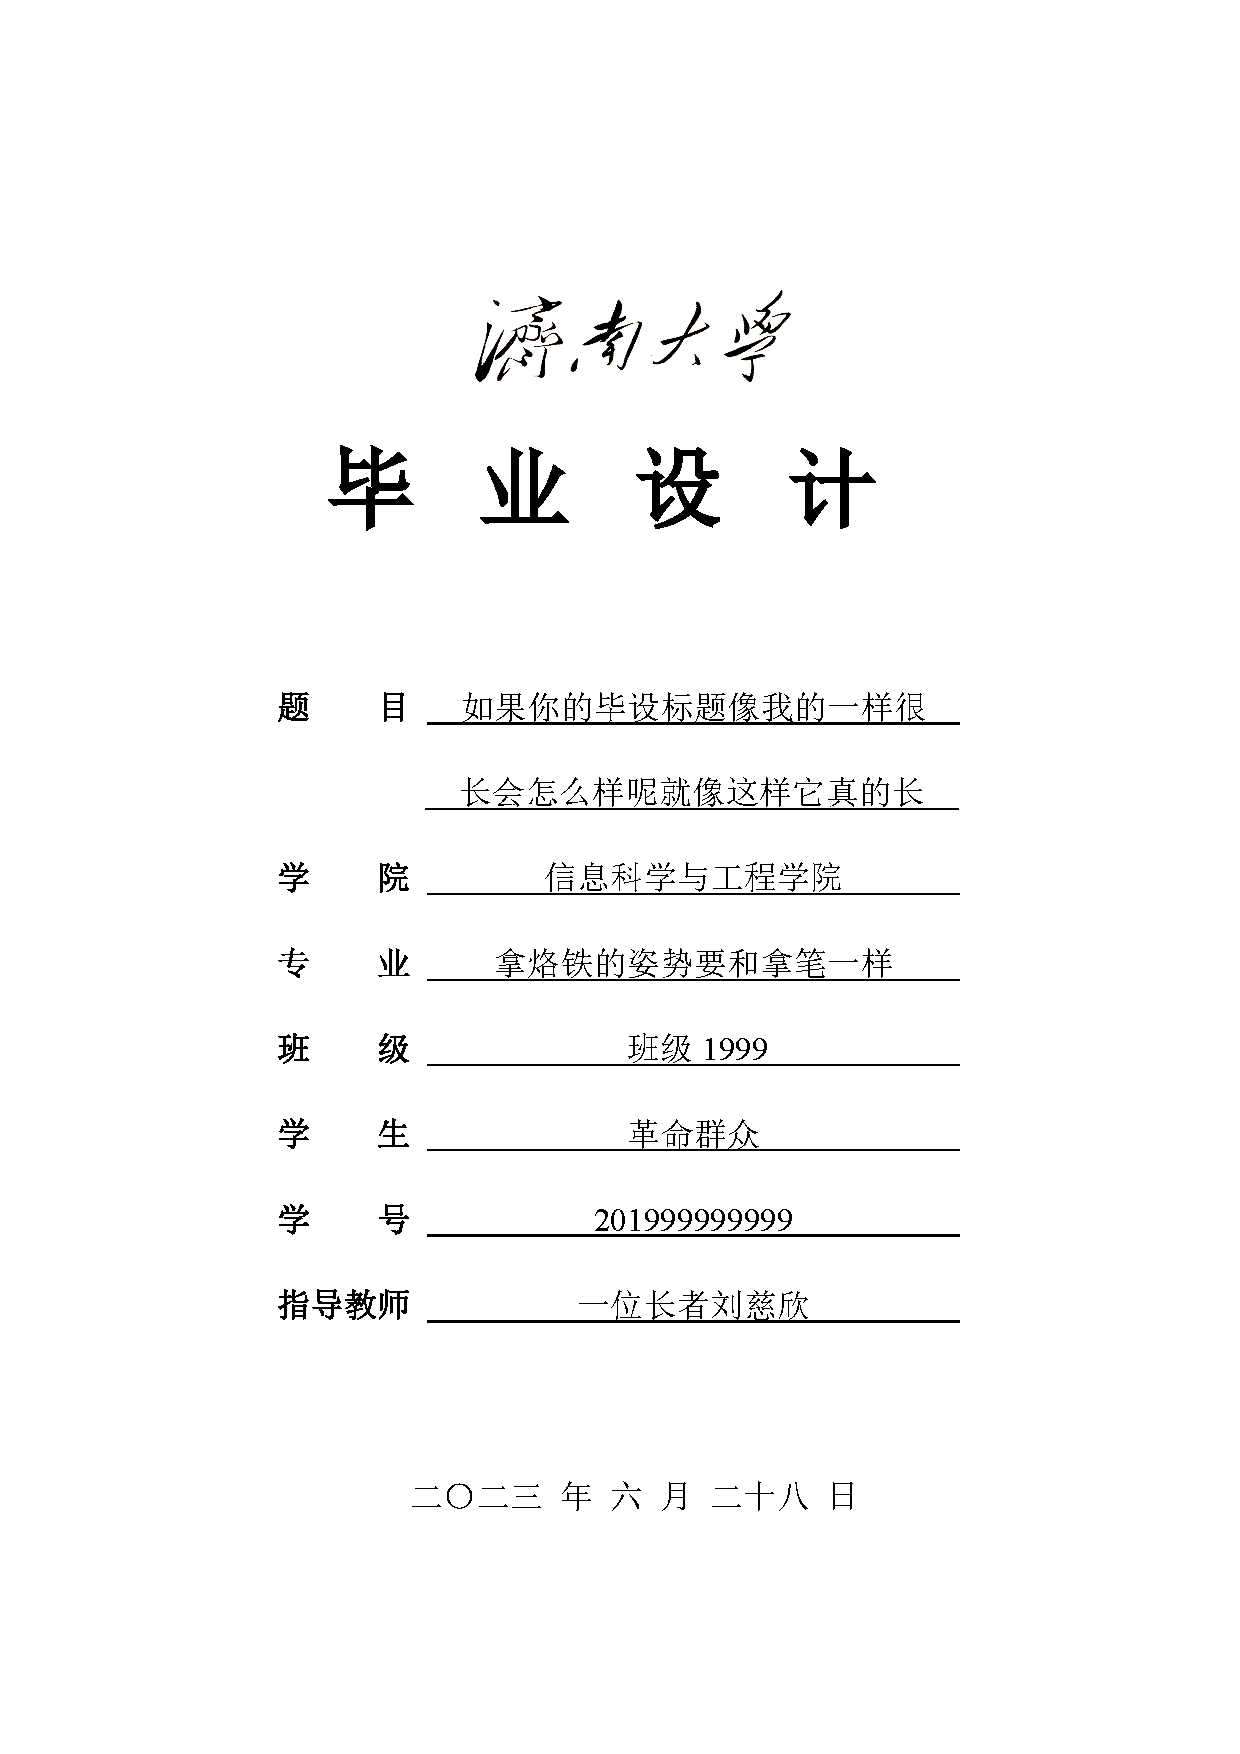
\includepdf[pages=-]{docs/01-cover.pdf}                     % 1 毕业论文封面


%%%%%%%%%%%%%%%%%%%%%%%%%% 以下为毕业论文正文内容 %%%%%%%%%%%%%%%%%%%%%%%%%%%%

\setblindingline
\setfancylength
\pagestyle{ujnabstract}
\begin{ujnabstract}
\section[摘要]{摘\qquad 要}
这是中文摘要的内容。
\end{ujnabstract}                 % 2.1 中文摘要
\pagestyle{ujnabstract*}
\begin{ujnabstract*}
\section{ABSTRACT}
\begin{spacing}{1.4}\normalsize{
% 以下为英文摘要内容,把点引线以下的文字替换成你的就好
% ·································································································
The University has established 4 national-level distinctive specialties,
5 national-level quality courses, 2 national-level exemplary bilingual courses,
2 national-level quality public audio and video courses,
6 specialties training for Outstanding Engineers, 16 provincial-level distinct specialties,
9 specialties jointly supported by the school and enterprise,
53 provincial-level top-grade courses and 5 provincial-level experimental teaching centers.
In recent years, the faculties have undertaken 6 national teaching and research projects and 55 provincial projects,
published 8 textbooks guided by China, and won 3 national "Teaching Achievements" awards and 75 provincial "Teaching and Research Achievements" awards.
In addition, the University has successively won a wide variety of honors for innovation and creativity,
such as the "Challenge Cup" Extracurricular and Academic Contest,
and China Undergraduate Mathematical Contest in Modeling.
The students have won 3133 provincial or national awards,
of which 48 are first prizes and 125 are second prizes at the national level.

In recent years, the university has undertaken 347 national research projects including funds from the National Science and Technology Support Program,
973 project program, 863 project program, and support from the Natural Science Foundation of China,
and Social Science Foundation of China, and 814 provincial projects.
The University has won 238 national and provincial prizes for research achievements,
one second prize of National Award for Technological Invention and 3 second prizes of National Award for Science and Technology Progress,
and obtained 666 national patents. 4799 papers were indexed by SCI, EI or ISTP. 214 academic works,
translations or textbooks were published. Eight journals are currently sponsored by the University of Jinan,
including "China Powder Science and Technology", "Chinese Journal of Cancer Prevention and Treatment",
and "Journal of University of Jinan".
% ·································································································
}\end{spacing}
\begin{spacing}{0.9}
% 以下为关键词的设置,把「keywordn」(n=1,2,3,...)替换成你的关键词就好
\small\enkeywords{congratulations;this is;jida}
\end{spacing}
\end{ujnabstract*}
                 % 2.2 英文摘要

\pagestyle{ujncontent}
这是 ch2-basic/content.tex 的内容。                     % 2.3 目录

\pagestyle{ujnbody}
\begin{ujnbody}
    \section{基础功能测试}
    \subsection{文字与段落}
    这是文字。

    这是段落。这是段落。这是段落。这是段落。这是段落。这是段落。这是段落。这是段落。这是段落。这是段落。这是段落。这是段落。这是段落。这是段落。这是段落。这是段落。这是段落。这是段落。
    \subsubsection{文字与段落}
    这是文字。

    这是段落。这是段落。这是段落。这是段落。这是段落。这是段落。这是段落。这是段落。这是段落。这是段落。这是段落。这是段落。这是段落。这是段落。这是段落。这是段落。这是段落。这是段落。
    \subsection{文字与段落}
    这是文字。

    这是段落。这是段落。这是段落。这是段落。这是段落。这是段落。这是段落。这是段落。这是段落。这是段落。这是段落。这是段落。这是段落。这是段落。这是段落。这是段落。这是段落。这是段落。
    \subsection{文字与段落}
    这是文字。

    这是段落。这是段落。这是段落。这是段落。这是段落。这是段落。这是段落。这是段落。这是段落。这是段落。这是段落。这是段落。这是段落。这是段落。这是段落。这是段落。这是段落。这是段落。
    \subsection{文字与段落}
    这是文字。

    这是段落。这是段落。这是段落。这是段落。这是段落。这是段落。这是段落。这是段落。这是段落。这是段落。这是段落。这是段落。这是段落。这是段落。这是段落。这是段落。这是段落。这是段落。
    \subsection{图表}

    \subsubsection{图片}

    \begin{figure}[htbp]
        \centering
        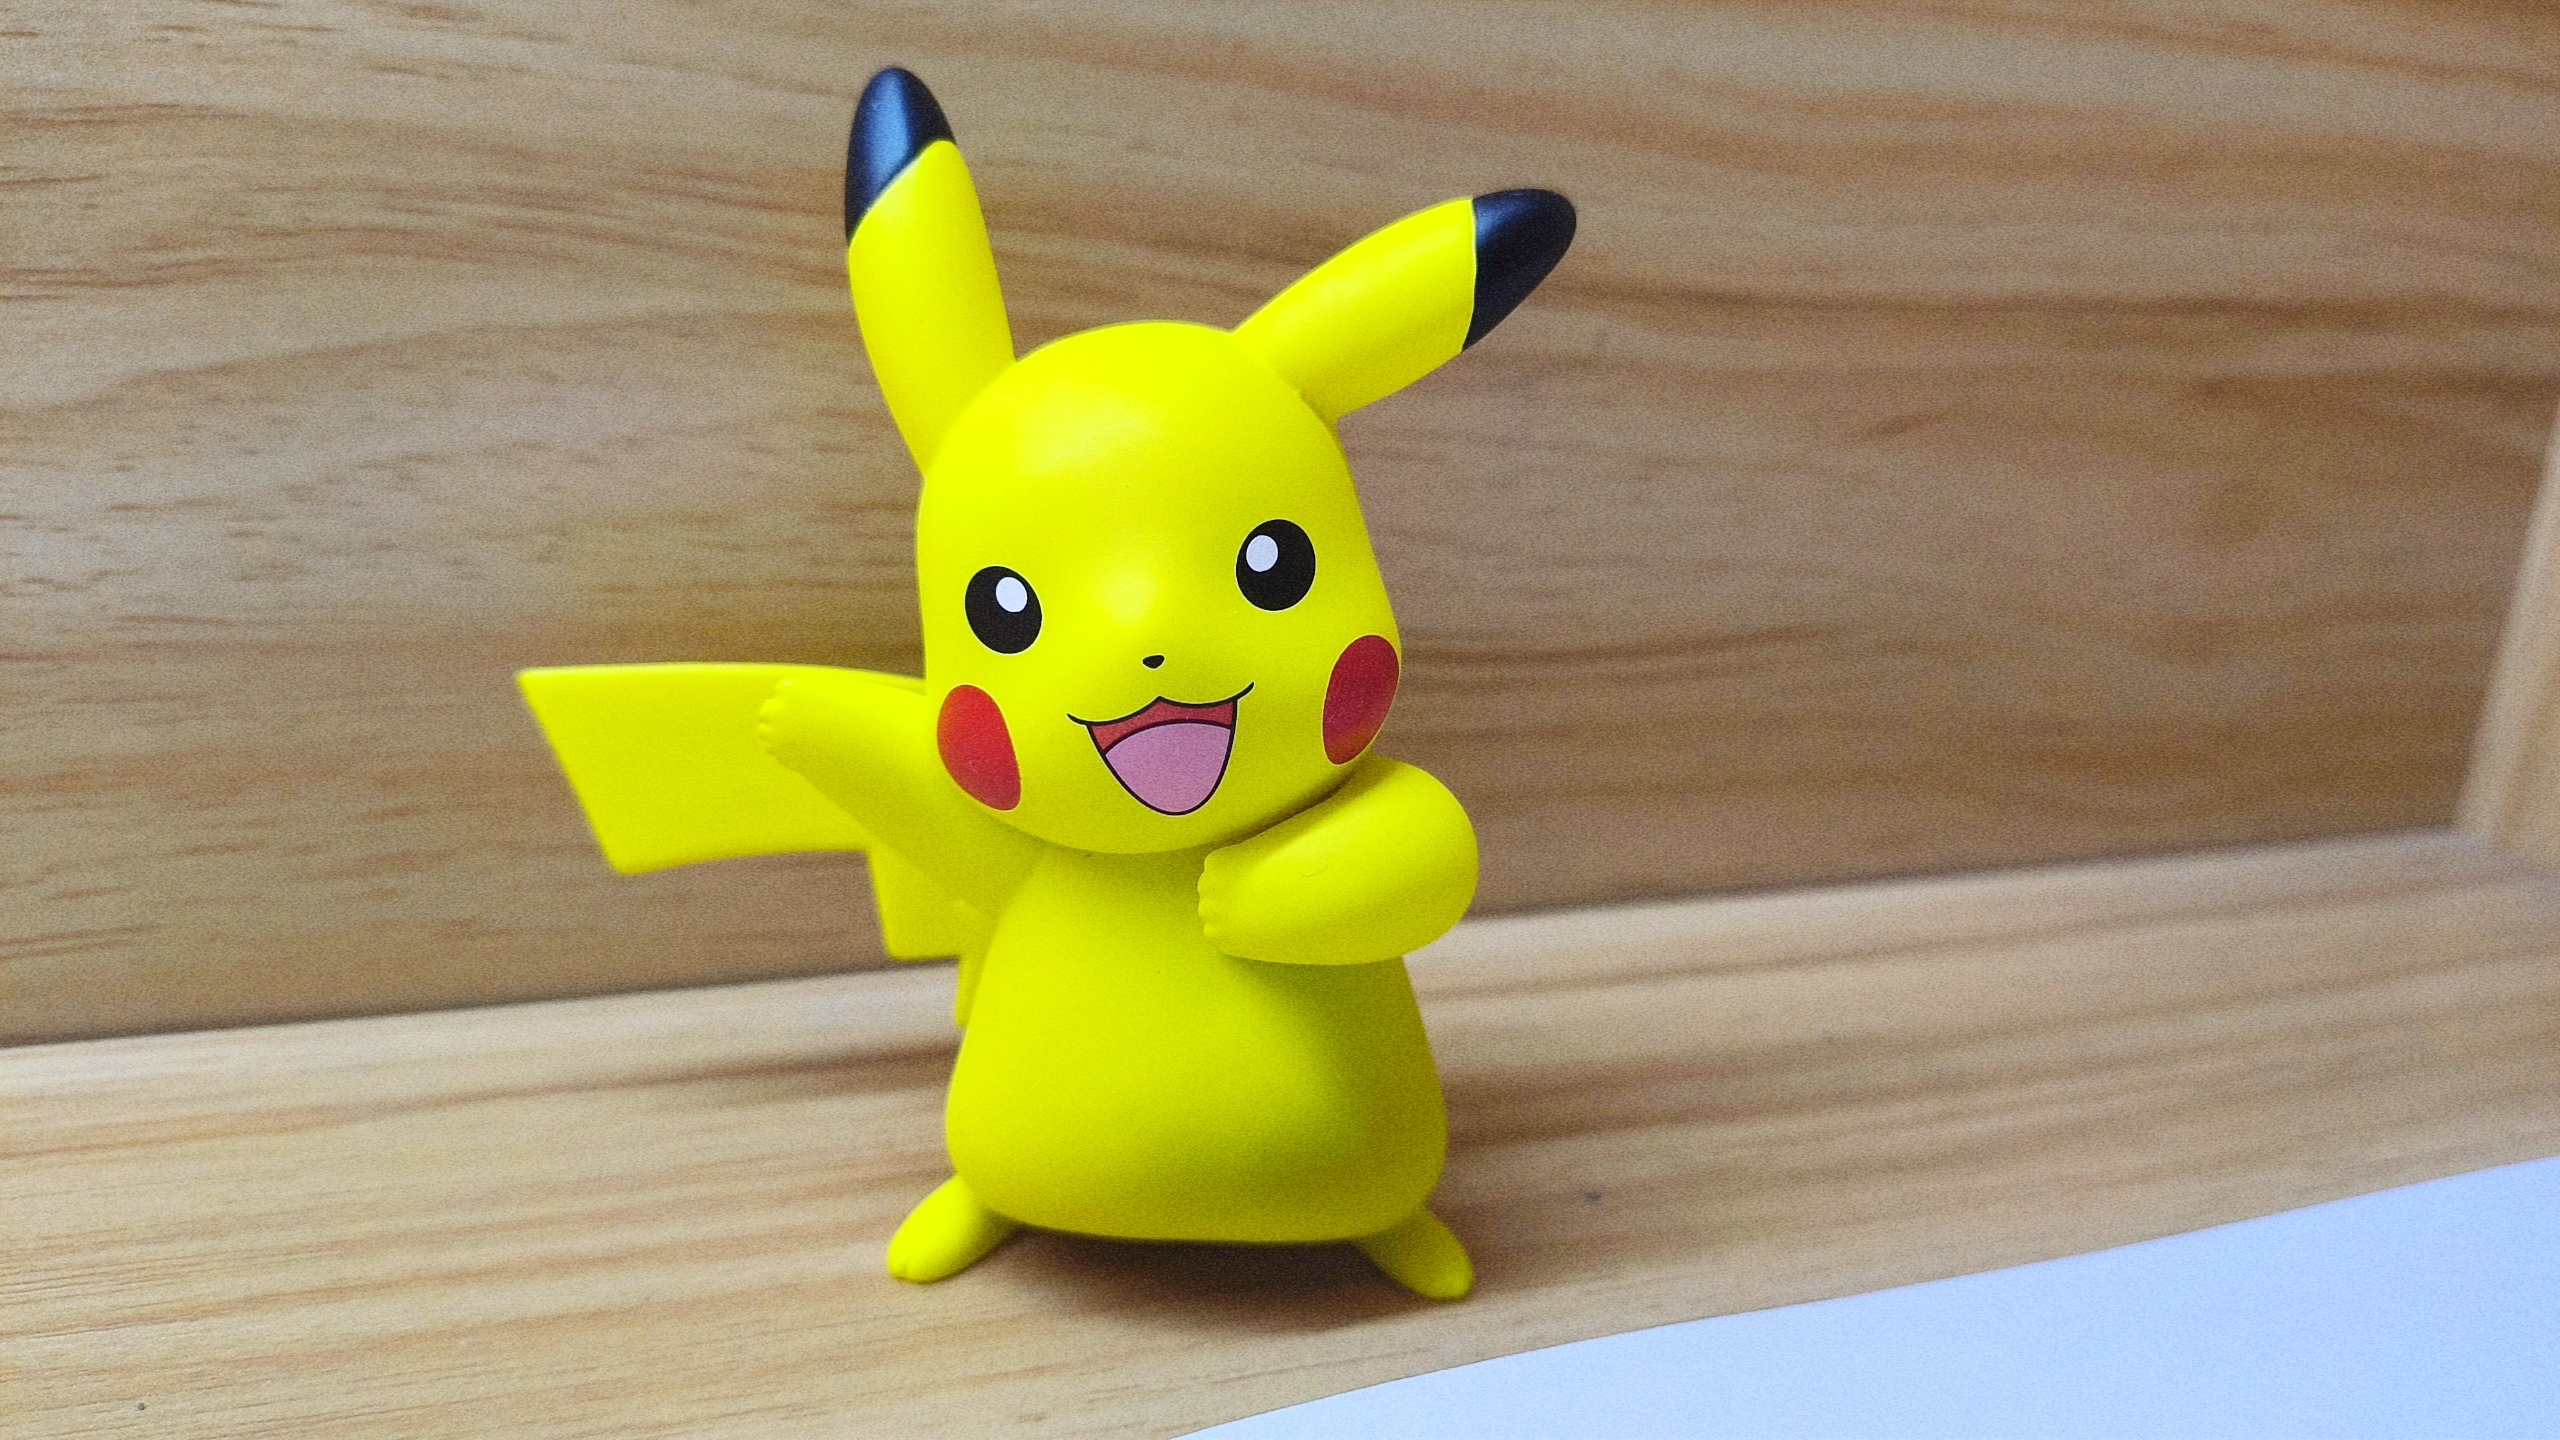
\includegraphics[scale=0.1, ]{figures/pikachu.jpg}
        \caption{这是图表}
        %\label{fig:1}
    \end{figure}

    \subsubsection{表格}

    \begin{table}[htbp]
        \centering
        \caption{这是表格}
        %\label{tab:1}
        \begin{tabular}{|c|c|c|}
            \hline
            \multicolumn{1}{|c|}{\textbf{表格}} & \multicolumn{1}{c|}{\textbf{表格}} & \multicolumn{1}{c|}{\textbf{表格}} \\ \hline
            \multicolumn{1}{|c|}{\textbf{表格}} & \multicolumn{1}{c|}{\textbf{表格}} & \multicolumn{1}{c|}{\textbf{表格}} \\ \hline
            \multicolumn{1}{|c|}{\textbf{表格}} & \multicolumn{1}{c|}{\textbf{表格}} & \multicolumn{1}{c|}{\textbf{表格}} \\ \hline
        \end{tabular}
    \end{table}
    \subsection{基础功能测试}
    \subsection{文字与段落}
    这是文字。

    这是段落。这是段落。这是段落。这是段落。这是段落。这是段落。这是段落。这是段落。这是段落。这是段落。这是段落。这是段落。这是段落。这是段落。这是段落。这是段落。这是段落。这是段落。
    \subsection{图表}

    \subsubsection{图片}

    \begin{figure}[htbp]
        \centering
        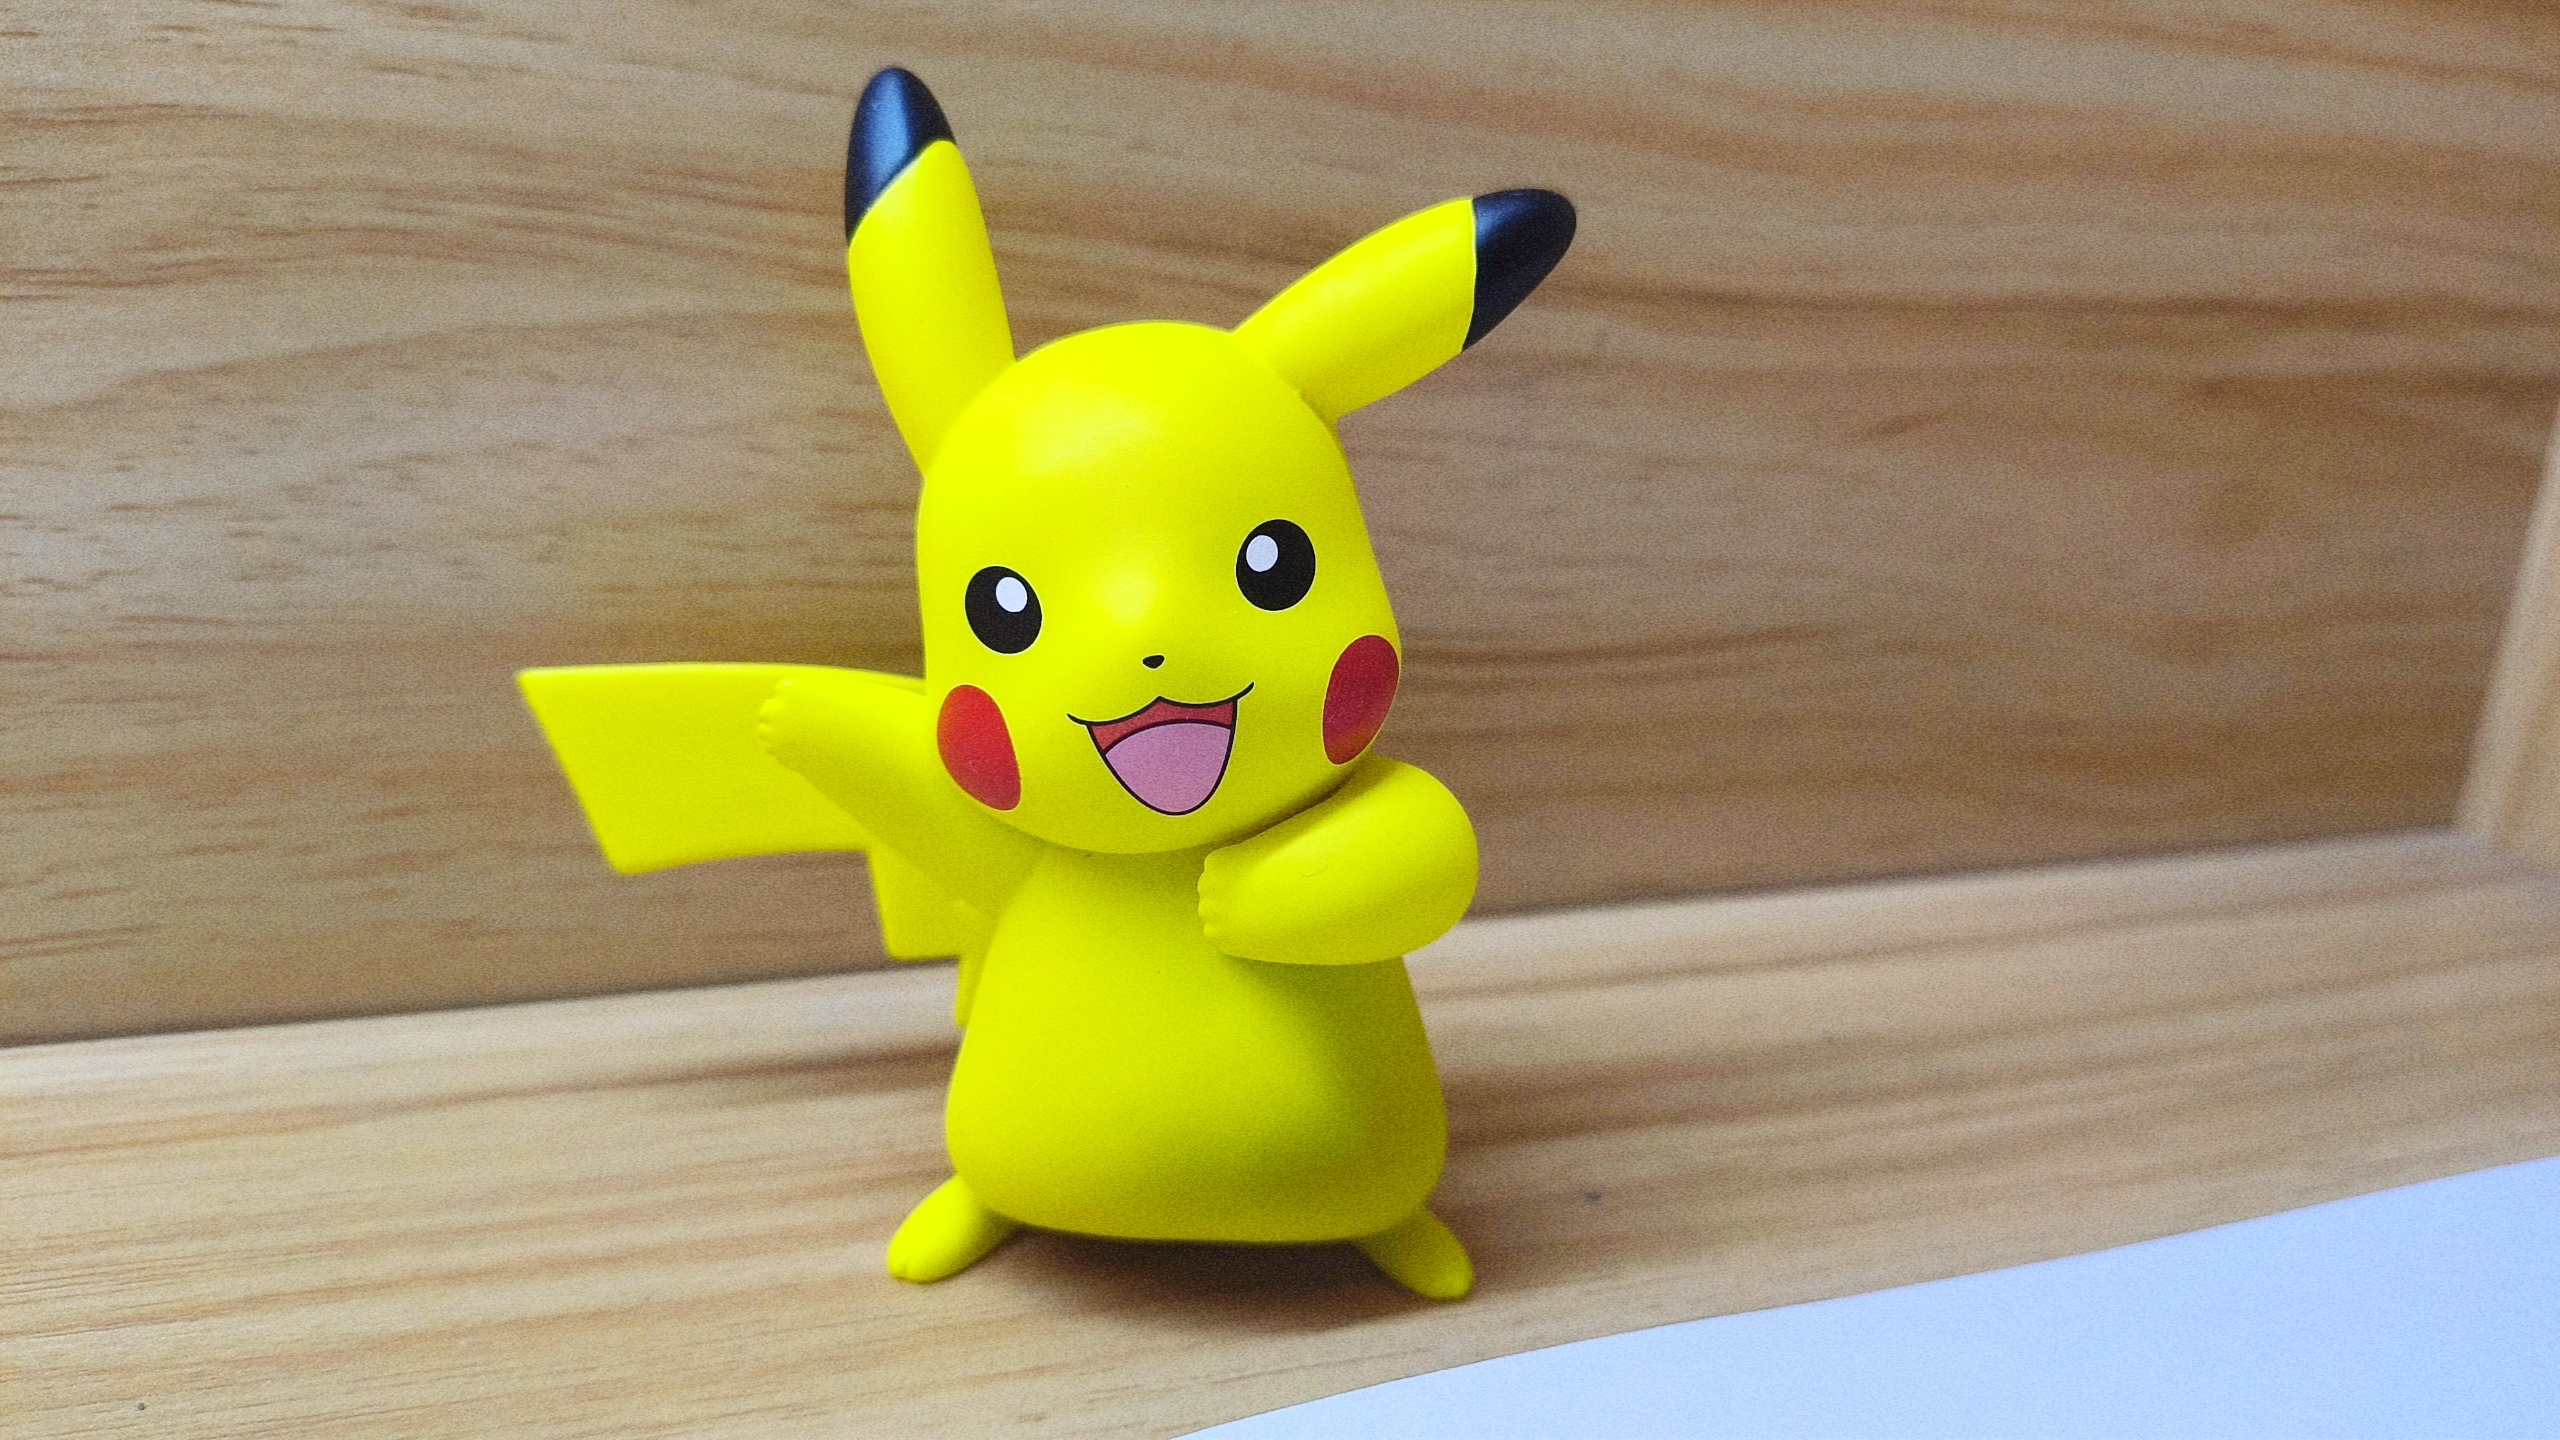
\includegraphics[scale=0.1, ]{figures/pikachu.jpg}
        \caption{这是图表}
        %\label{fig:1}
    \end{figure}

    \subsubsection{表格}

    \begin{table}[htbp]
        \centering
        \caption{这是表格}
        %\label{tab:1}
        \begin{tabular}{|c|c|c|}
            \hline
            \multicolumn{1}{|c|}{\textbf{表格}} & \multicolumn{1}{c|}{\textbf{表格}} & \multicolumn{1}{c|}{\textbf{表格}} \\ \hline
            \multicolumn{1}{|c|}{\textbf{表格}} & \multicolumn{1}{c|}{\textbf{表格}} & \multicolumn{1}{c|}{\textbf{表格}} \\ \hline
            \multicolumn{1}{|c|}{\textbf{表格}} & \multicolumn{1}{c|}{\textbf{表格}} & \multicolumn{1}{c|}{\textbf{表格}} \\ \hline
        \end{tabular}
    \end{table}
    \subsection{基础功能测试}
    \subsection{文字与段落}
    这是文字。

    这是段落。这是段落。这是段落。这是段落。这是段落。这是段落。这是段落。这是段落。这是段落。这是段落。这是段落。这是段落。这是段落。这是段落。这是段落。这是段落。这是段落。这是段落。
    \subsection{文字与段落}
    这是文字。

    这是段落。这是段落。这是段落。这是段落。这是段落。这是段落。这是段落。这是段落。这是段落。这是段落。这是段落。这是段落。这是段落。这是段落。这是段落。这是段落。这是段落。这是段落。
    \subsection{文字与段落}
    这是文字。

    这是段落。这是段落。这是段落。这是段落。这是段落。这是段落。这是段落。这是段落。这是段落。这是段落。这是段落。这是段落。这是段落。这是段落。这是段落。这是段落。这是段落。这是段落。
    \subsection{文字与段落}
    这是文字。

    这是段落。这是段落。这是段落。这是段落。这是段落。这是段落。这是段落。这是段落。这是段落。这是段落。这是段落。这是段落。这是段落。这是段落。这是段落。这是段落。这是段落。这是段落。
    \subsection{图表}

    \subsubsection{图片}

    \begin{figure}[htbp]
        \centering
        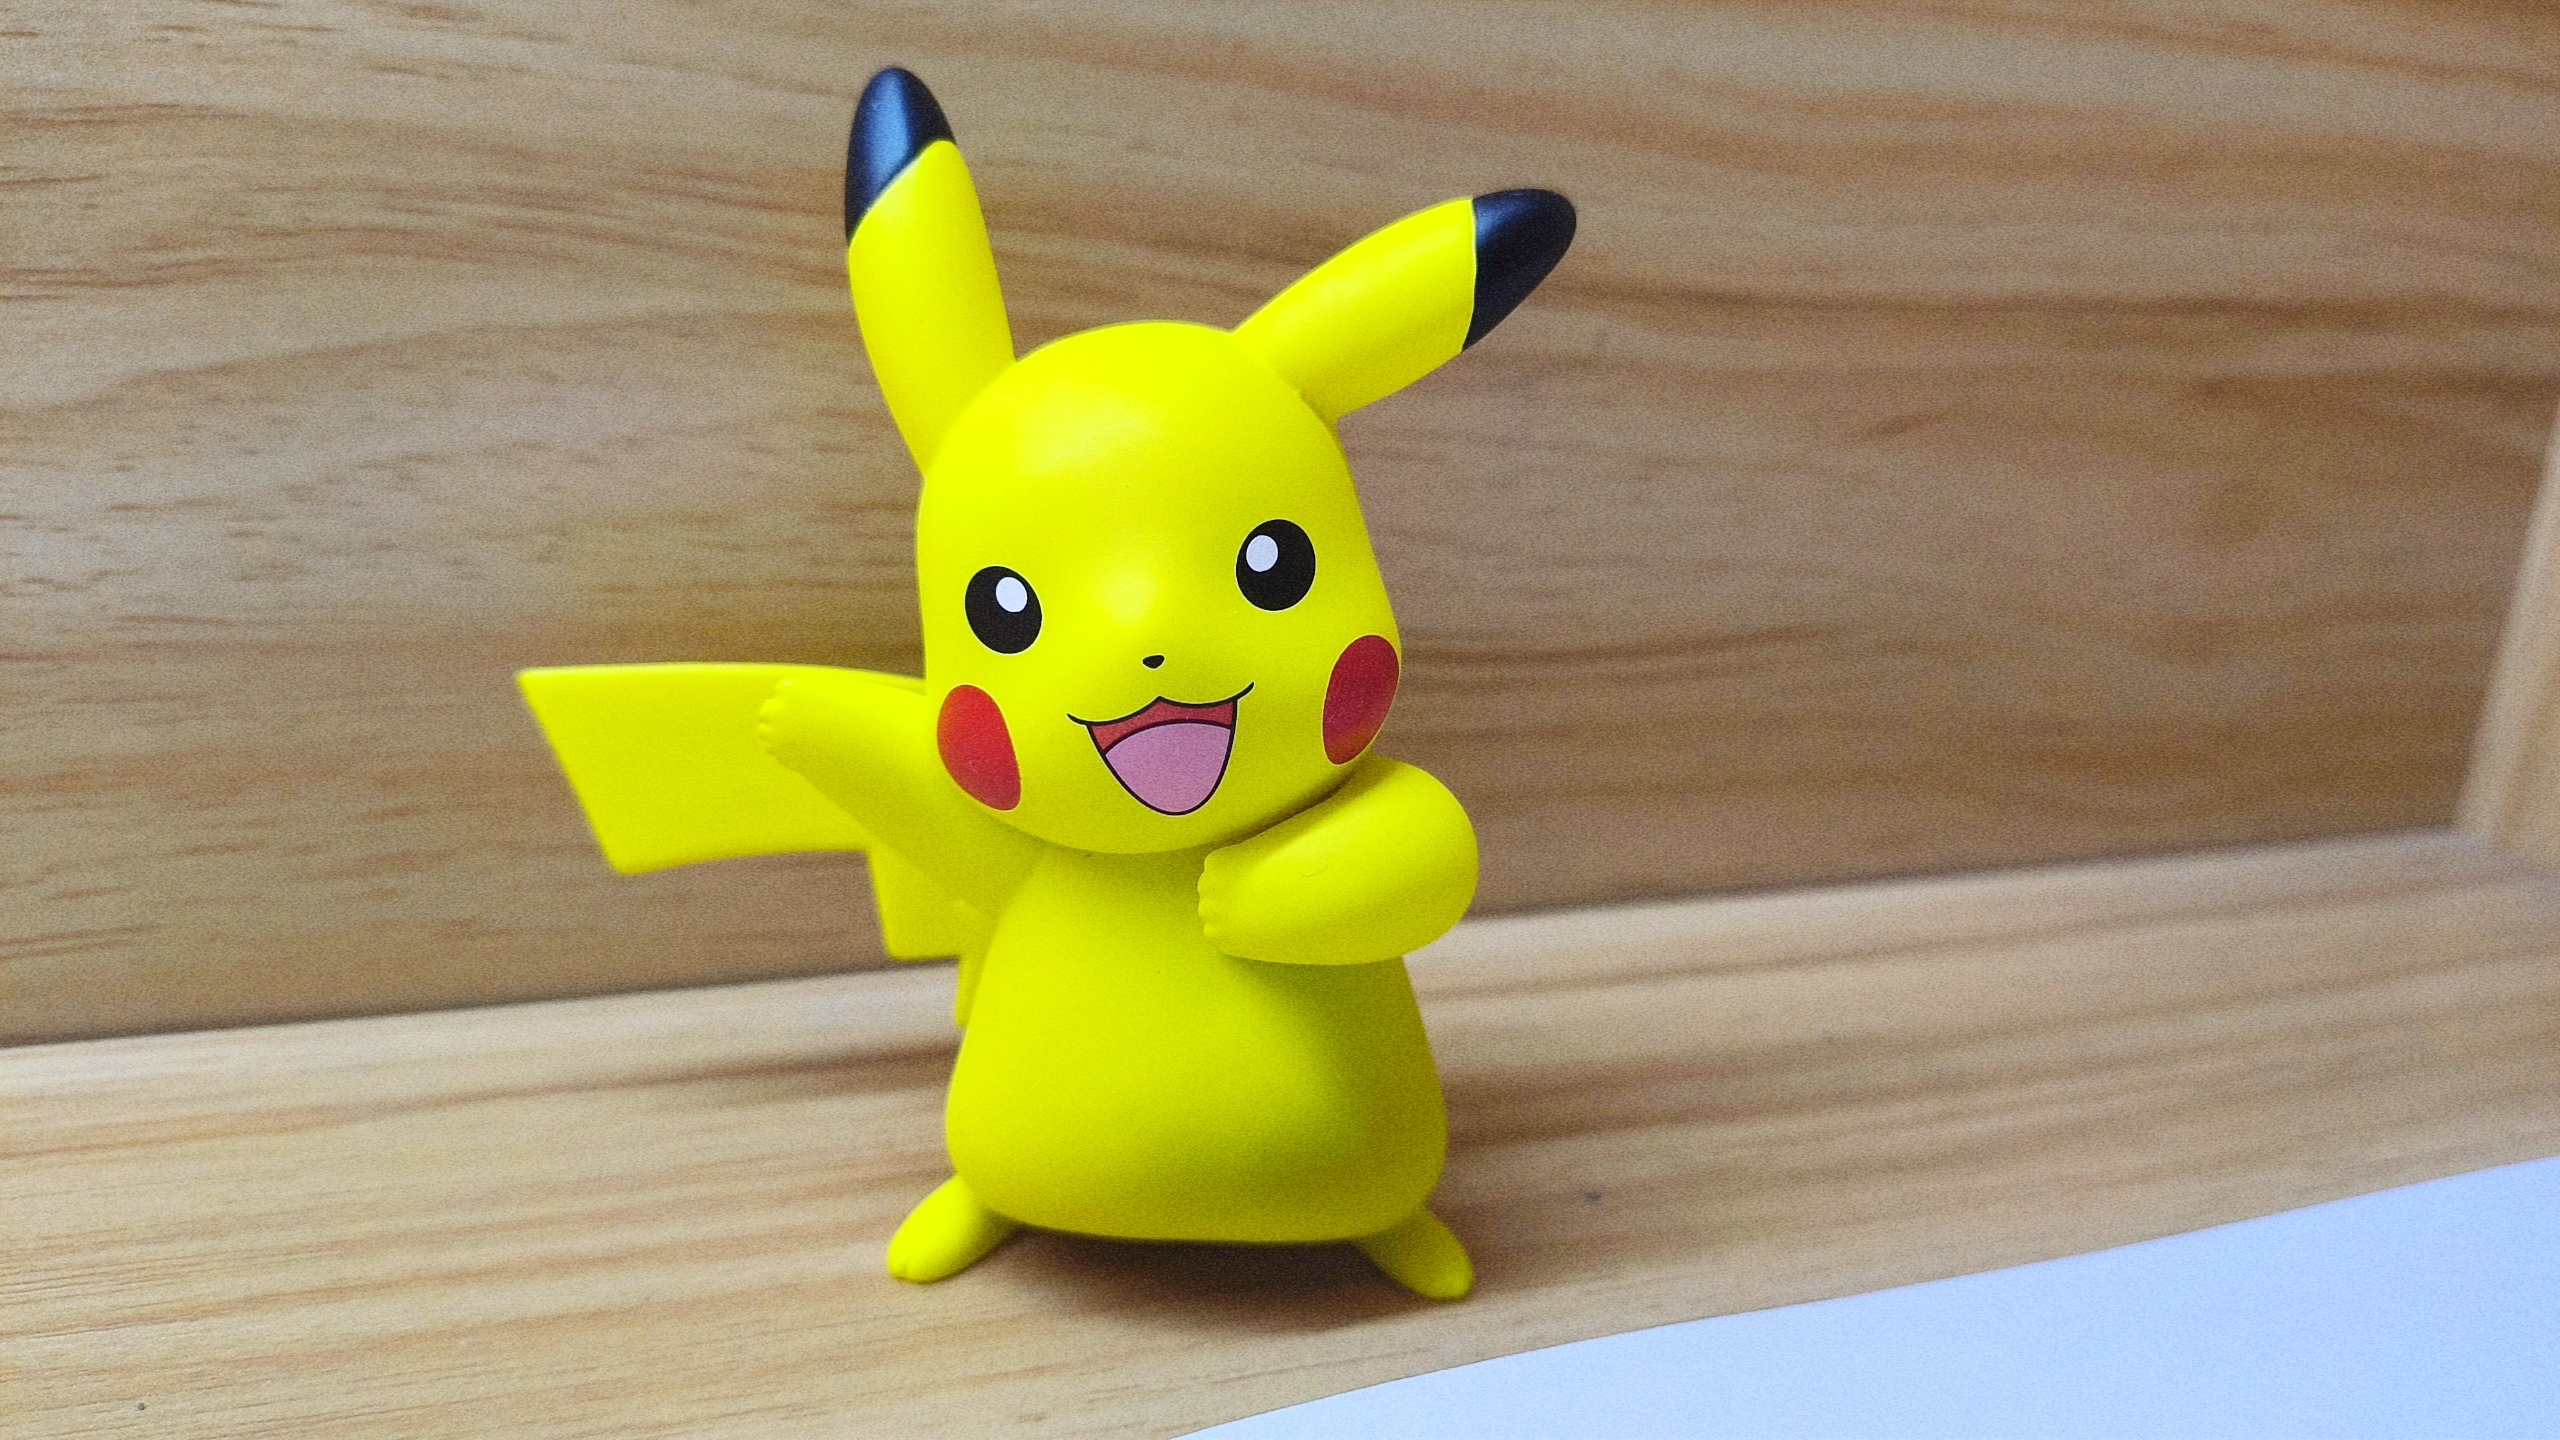
\includegraphics[scale=0.1, ]{figures/pikachu.jpg}
        \caption{这是图表}
        %\label{fig:1}
    \end{figure}

    \subsubsection{表格}

    \begin{table}[htbp]
        \centering
        \caption{这是表格}
        %\label{tab:1}
        \begin{tabular}{|c|c|c|}
            \hline
            \multicolumn{1}{|c|}{\textbf{表格}} & \multicolumn{1}{c|}{\textbf{表格}} & \multicolumn{1}{c|}{\textbf{表格}} \\ \hline
            \multicolumn{1}{|c|}{\textbf{表格}} & \multicolumn{1}{c|}{\textbf{表格}} & \multicolumn{1}{c|}{\textbf{表格}} \\ \hline
            \multicolumn{1}{|c|}{\textbf{表格}} & \multicolumn{1}{c|}{\textbf{表格}} & \multicolumn{1}{c|}{\textbf{表格}} \\ \hline
        \end{tabular}
    \end{table}
    \section{基础功能测试}
    \subsection{文字与段落}
    这是文字。

    这是段落。这是段落。这是段落。这是段落。这是段落。这是段落。这是段落。这是段落。这是段落。这是段落。这是段落。这是段落。这是段落。这是段落。这是段落。这是段落。这是段落。这是段落。
    \subsection{图表}

    \subsubsection{图片}

    \begin{figure}[htbp]
        \centering
        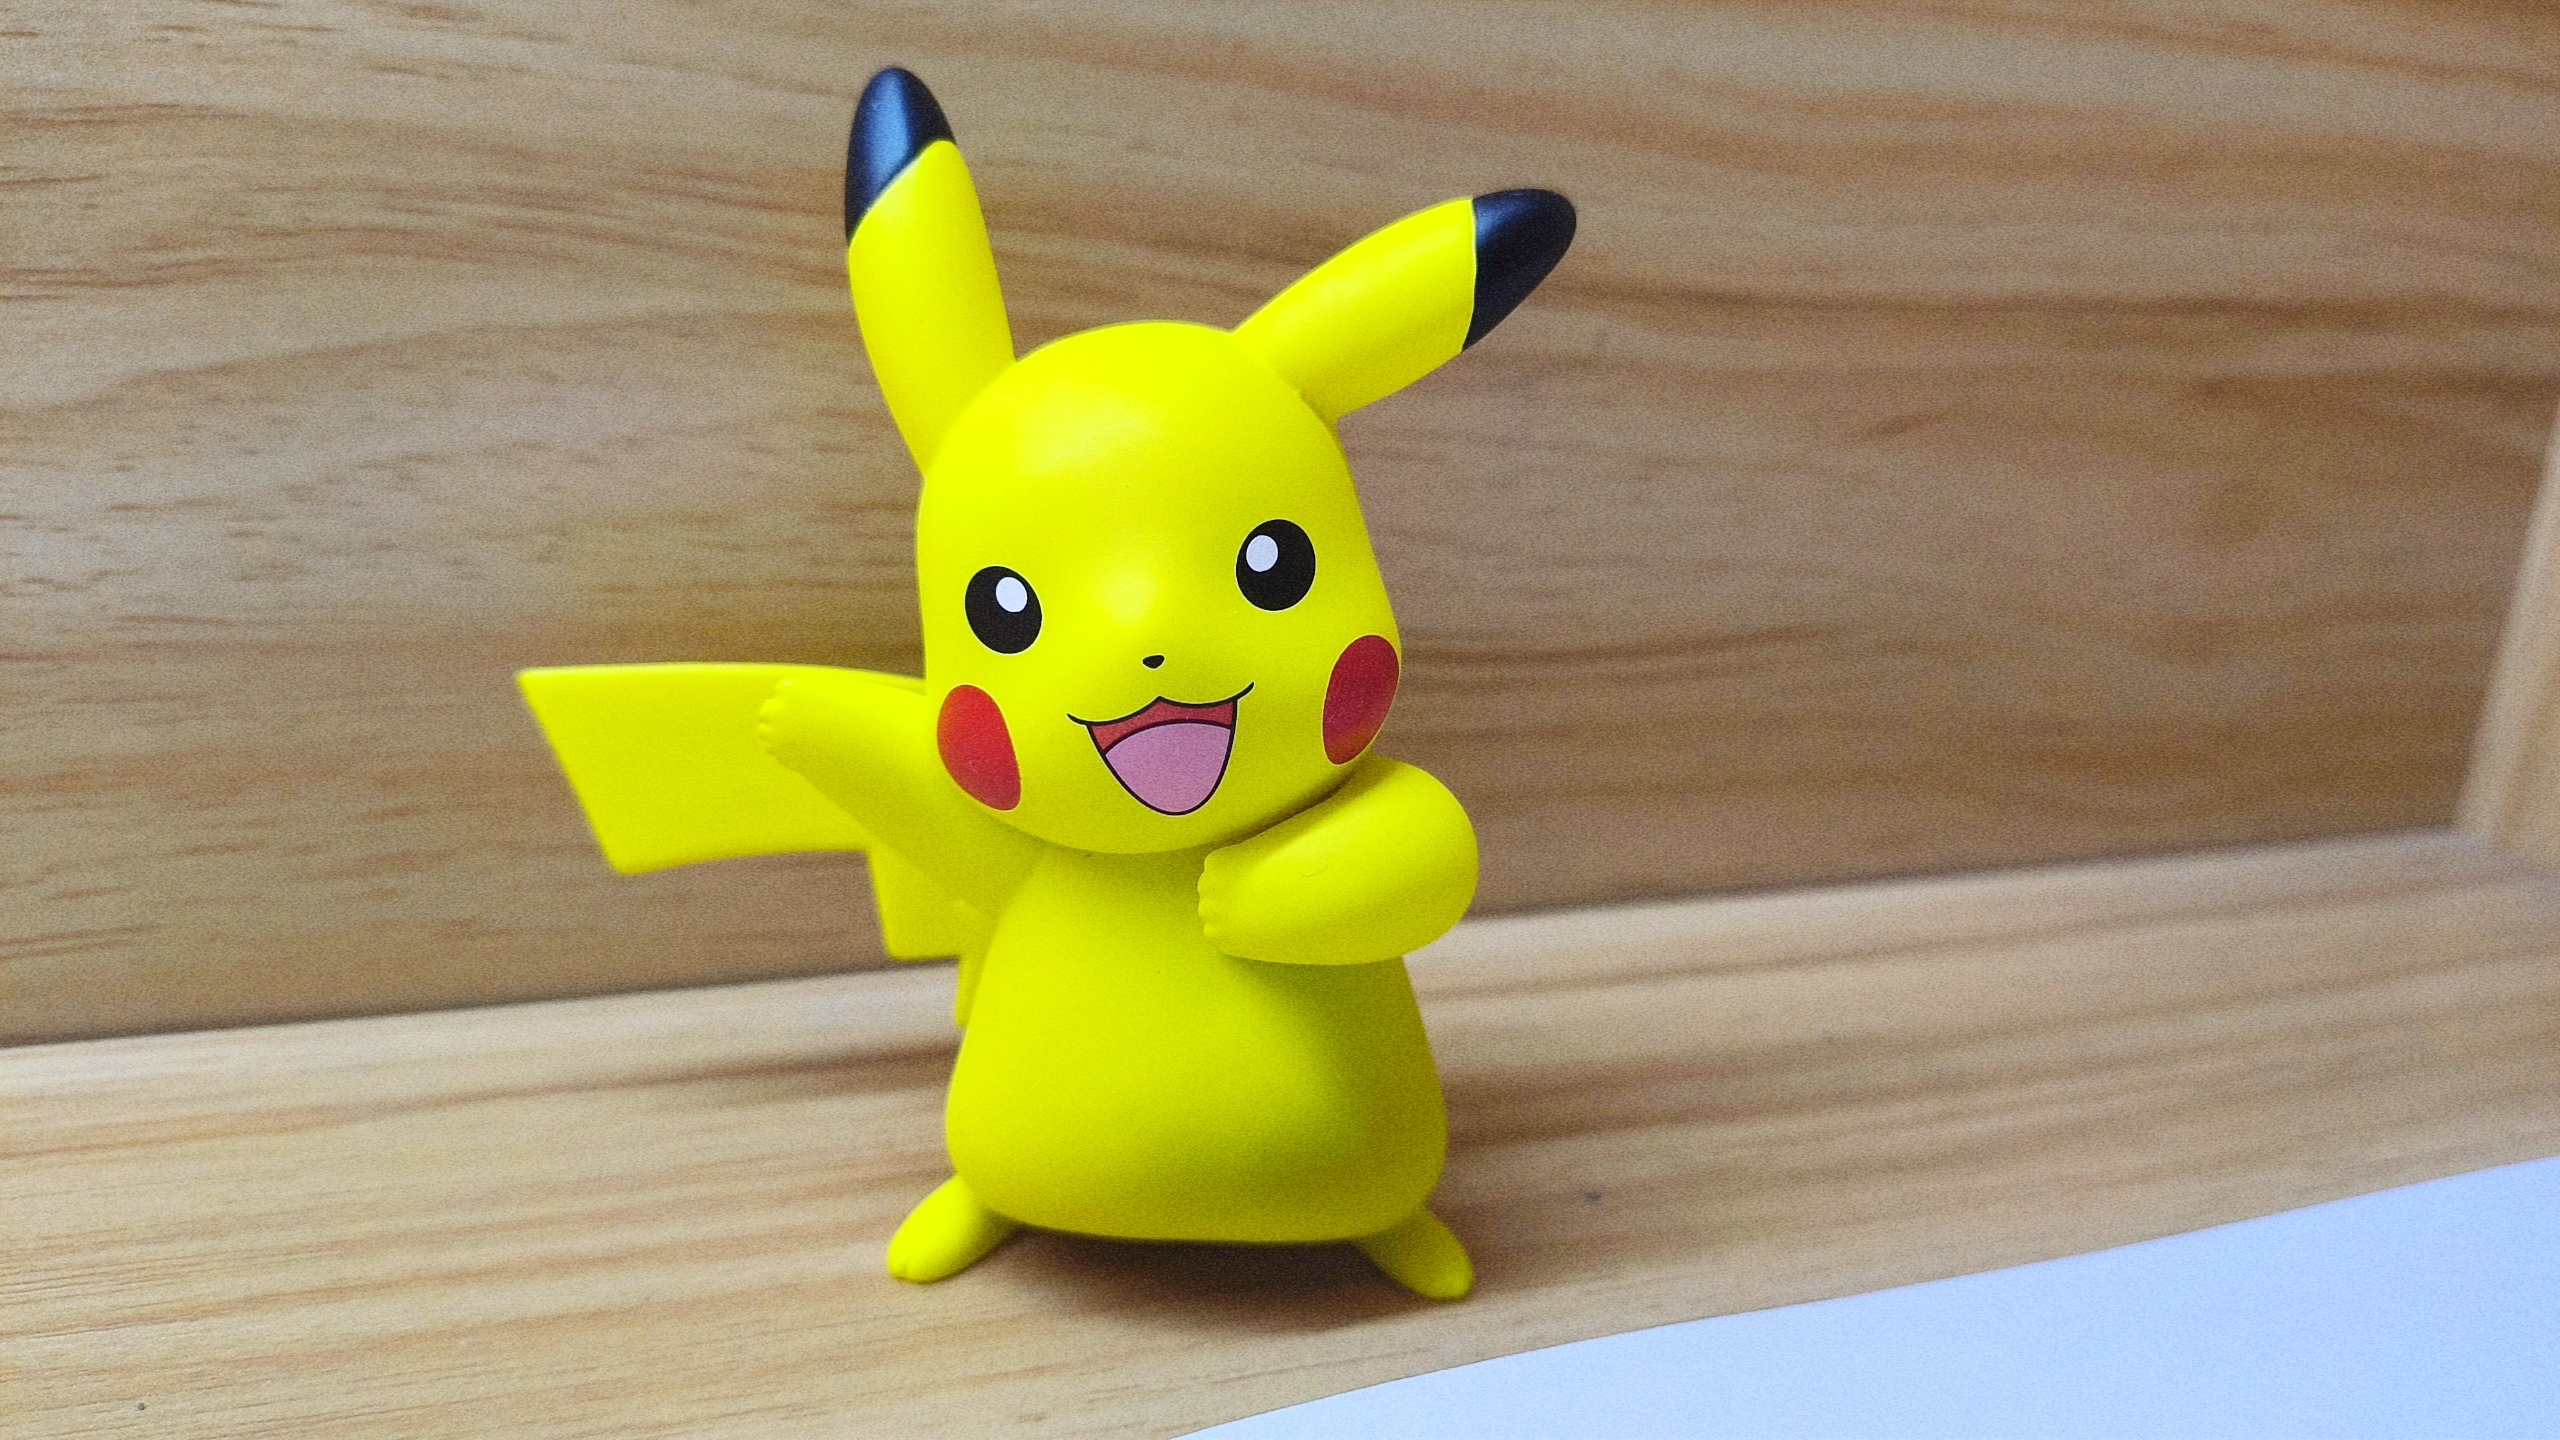
\includegraphics[scale=0.1, ]{figures/pikachu.jpg}
        \caption{这是图表}
        %\label{fig:1}
    \end{figure}

    \subsubsection{表格}

    \begin{table}[htbp]
        \centering
        \caption{这是表格}
        %\label{tab:1}
        \begin{tabular}{|c|c|c|}
            \hline
            \multicolumn{1}{|c|}{\textbf{表格}} & \multicolumn{1}{c|}{\textbf{表格}} & \multicolumn{1}{c|}{\textbf{表格}} \\ \hline
            \multicolumn{1}{|c|}{\textbf{表格}} & \multicolumn{1}{c|}{\textbf{表格}} & \multicolumn{1}{c|}{\textbf{表格}} \\ \hline
            \multicolumn{1}{|c|}{\textbf{表格}} & \multicolumn{1}{c|}{\textbf{表格}} & \multicolumn{1}{c|}{\textbf{表格}} \\ \hline
        \end{tabular}
    \end{table}
\end{ujnbody}                        % 2.4 正文

\pagestyle{ujnothers}
\chapter*{结论}
这是 ch2-basic/conclusion.tex 的内容。                  % 2.5 结论
\begin{ujnreference}
\section[参考文献]{参\enspace 考\enspace 文\enspace 献}
这是 ch2-basic/reference.tex 的内容。
\end{ujnreference}
                   % 2.6 参考文献
\begin{ujnthanks}
\chapter[致谢]{致\qquad 谢}
这是 ch2-basic/thanks.tex 的内容。
\end{ujnthanks}
                      % 2.7 致谢
\begin{ujnappendix}
\section[附录]{附\qquad 录}
% 以下为附录,把点引线以下的文字替换成你的就好
% ·································································································
    \subsection*{附录A 计算机的层次模型}
        \begin{figure}[htbp]
            \centering
            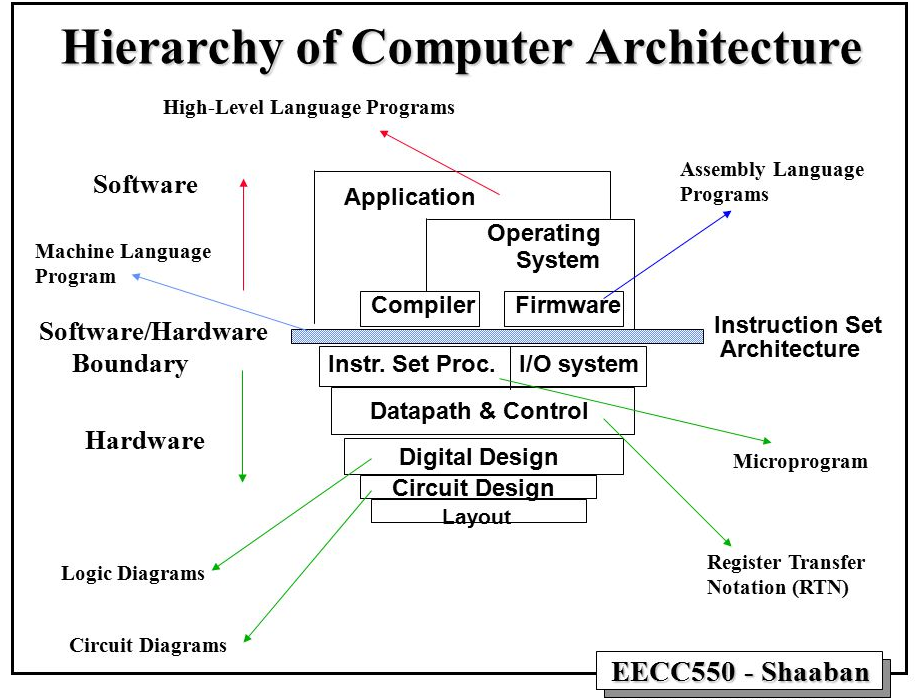
\includegraphics[width=0.8\textwidth]{figures/computer-arch.png}
            \caption{计算机的层次模型}
            \label{fig:computer-arch}
        \end{figure}
    \subsection*{附录B RV32I Base Integer Instruction Set}
% ·································································································
\end{ujnappendix}
                    % 2.8 附录
\unsetblindingline
\unsetfancylength

%%%%%%%%%%%%%%%%%%%%%%%%%% 以上为毕业论文正文内容 %%%%%%%%%%%%%%%%%%%%%%%%%%%%

% 3-6 表格性质的其他内容
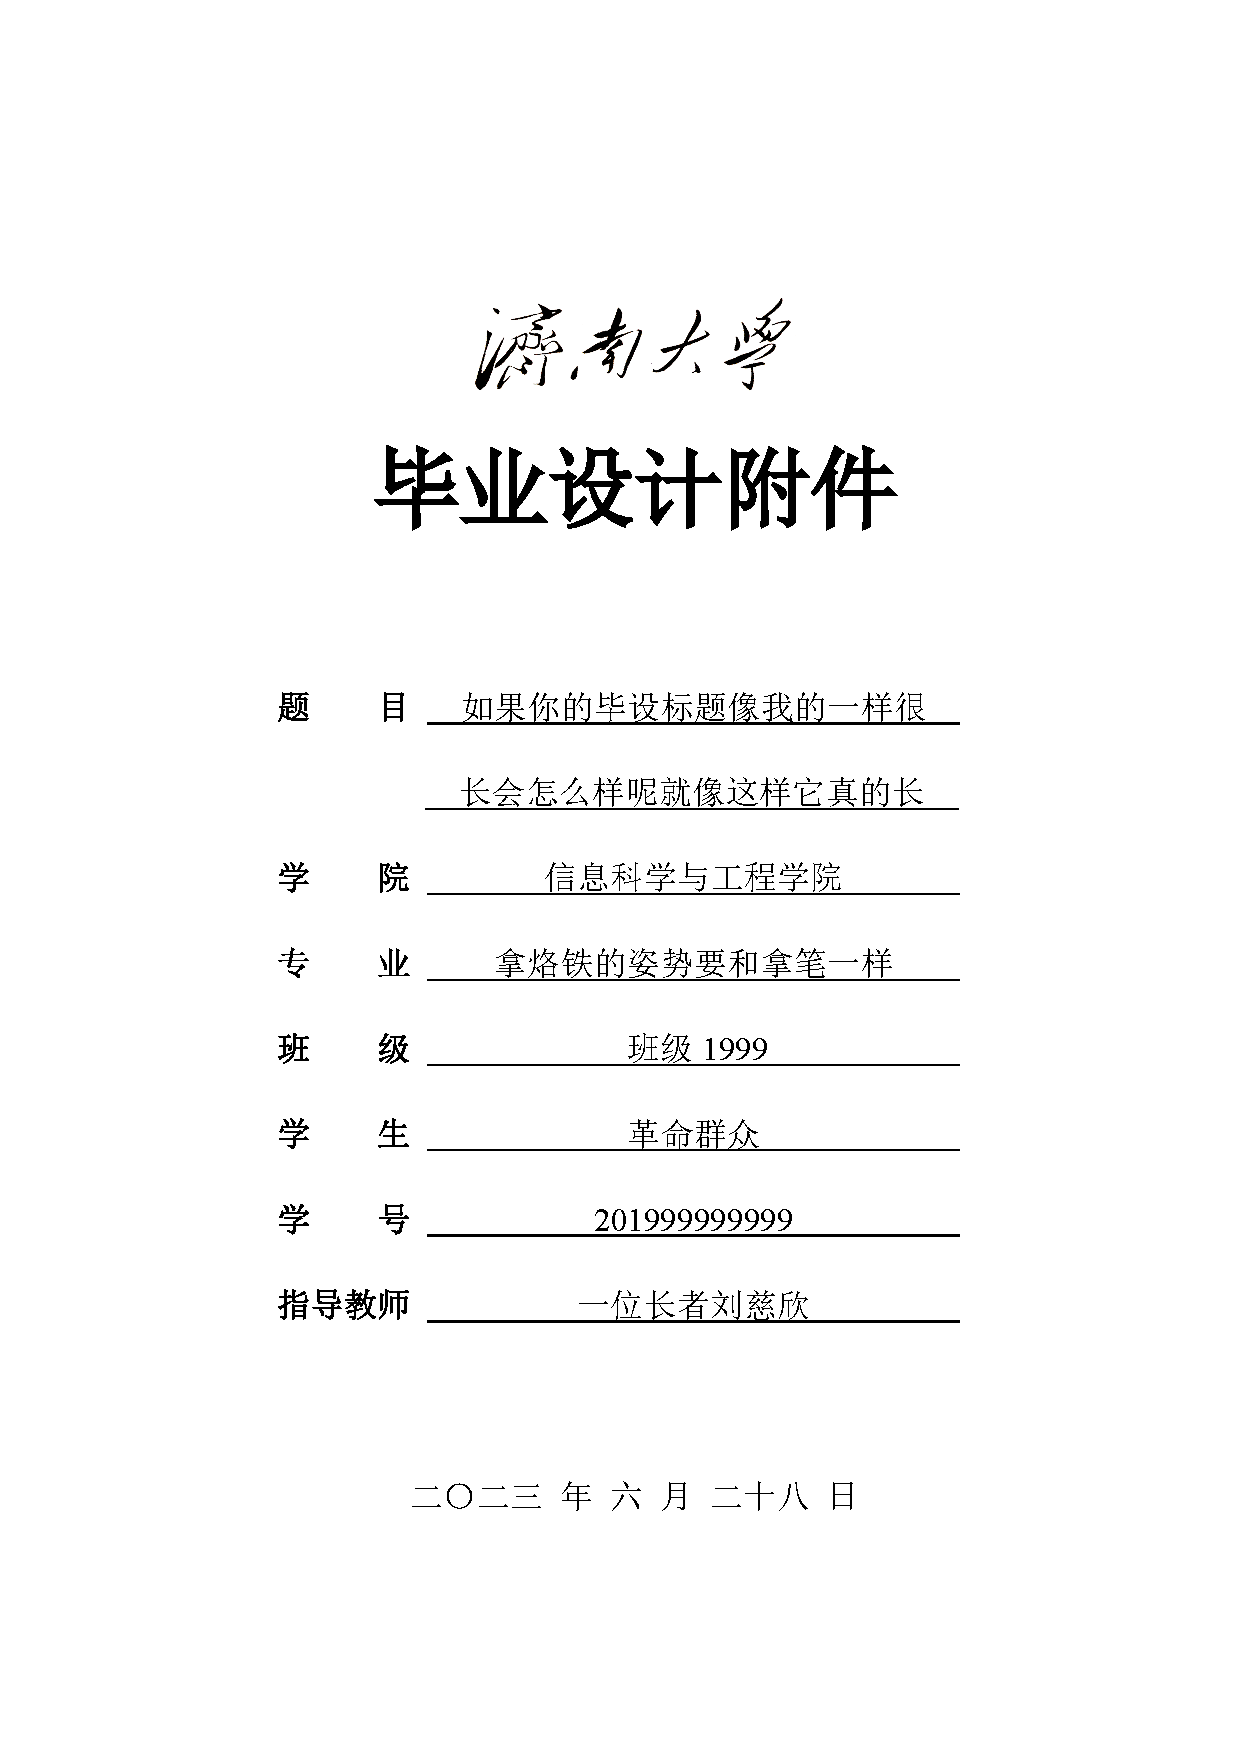
\includepdf[pages=-]{docs/03-appendix-cover.pdf}
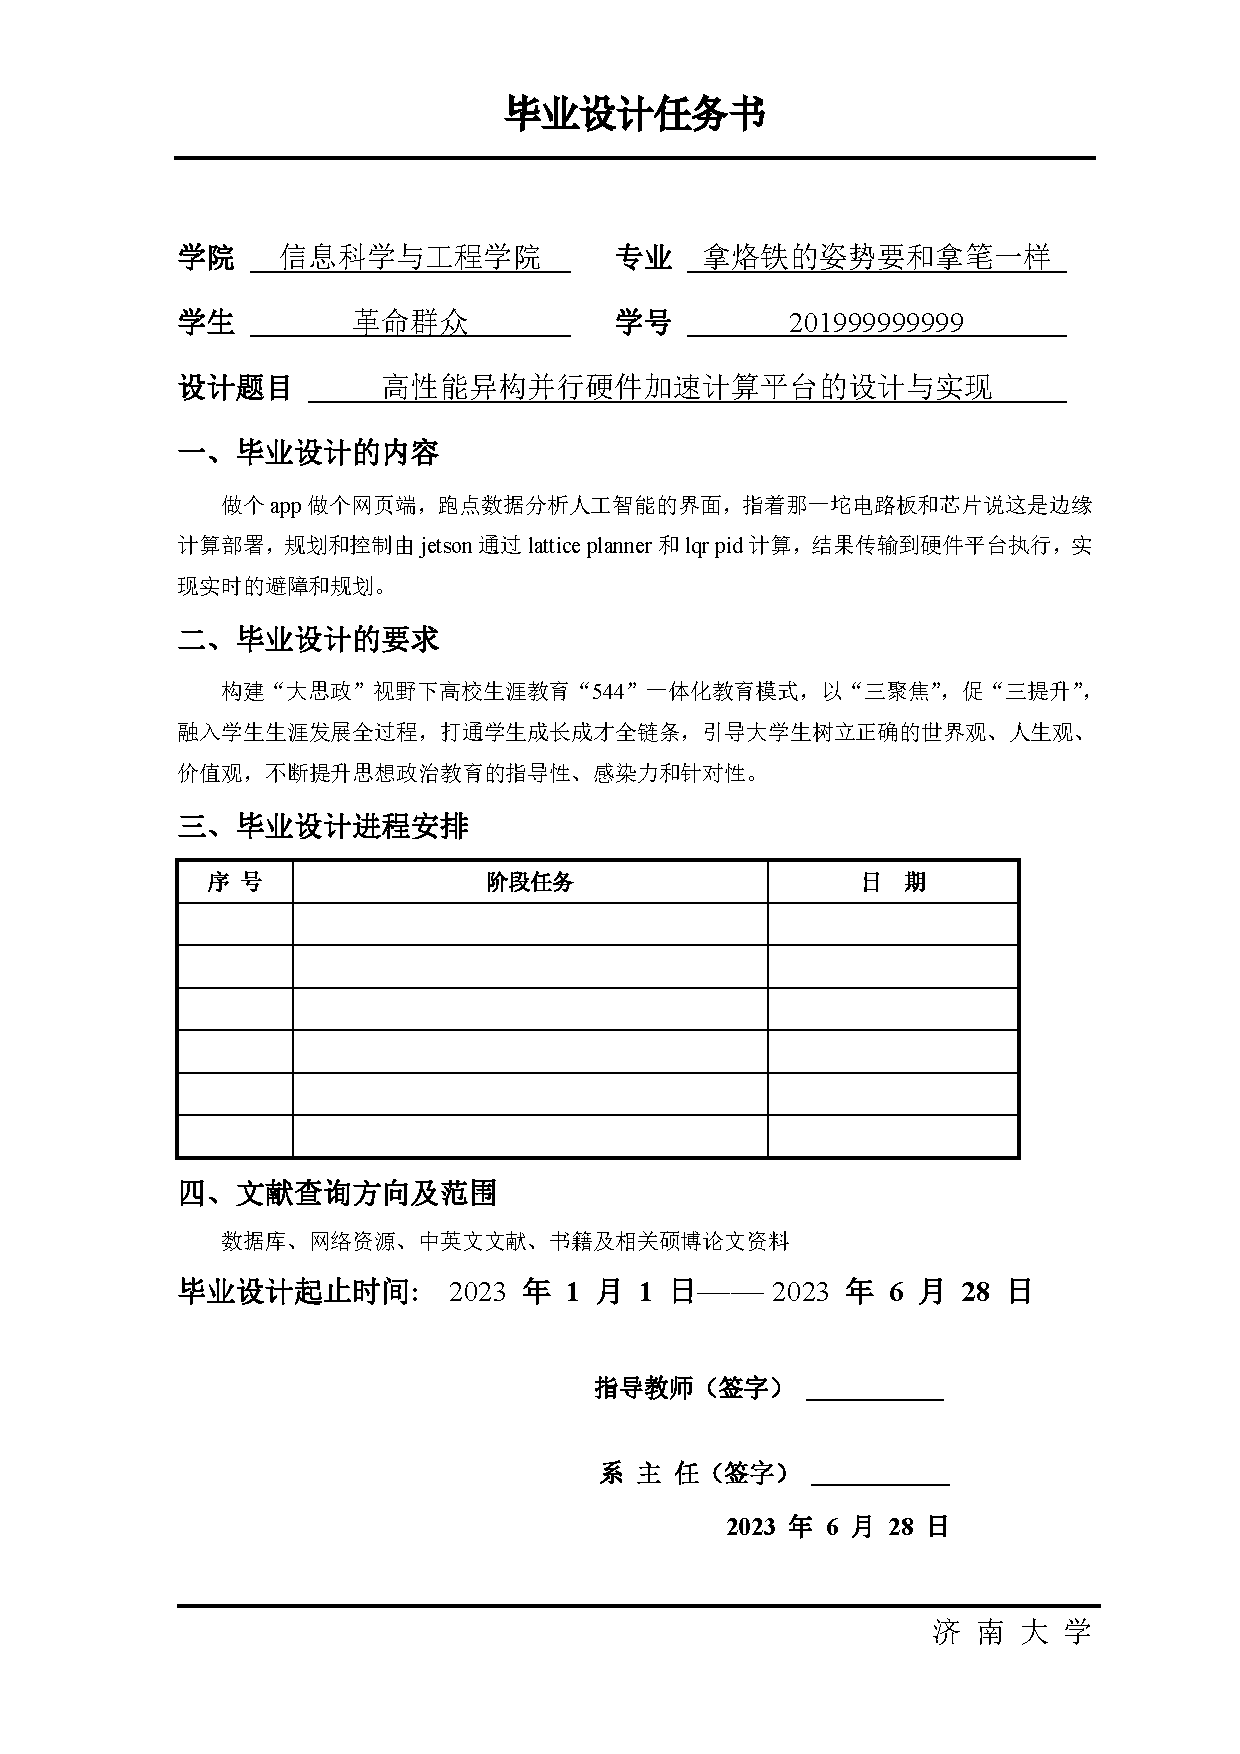
\includepdf[pages=-]{docs/04-taskbook.pdf}
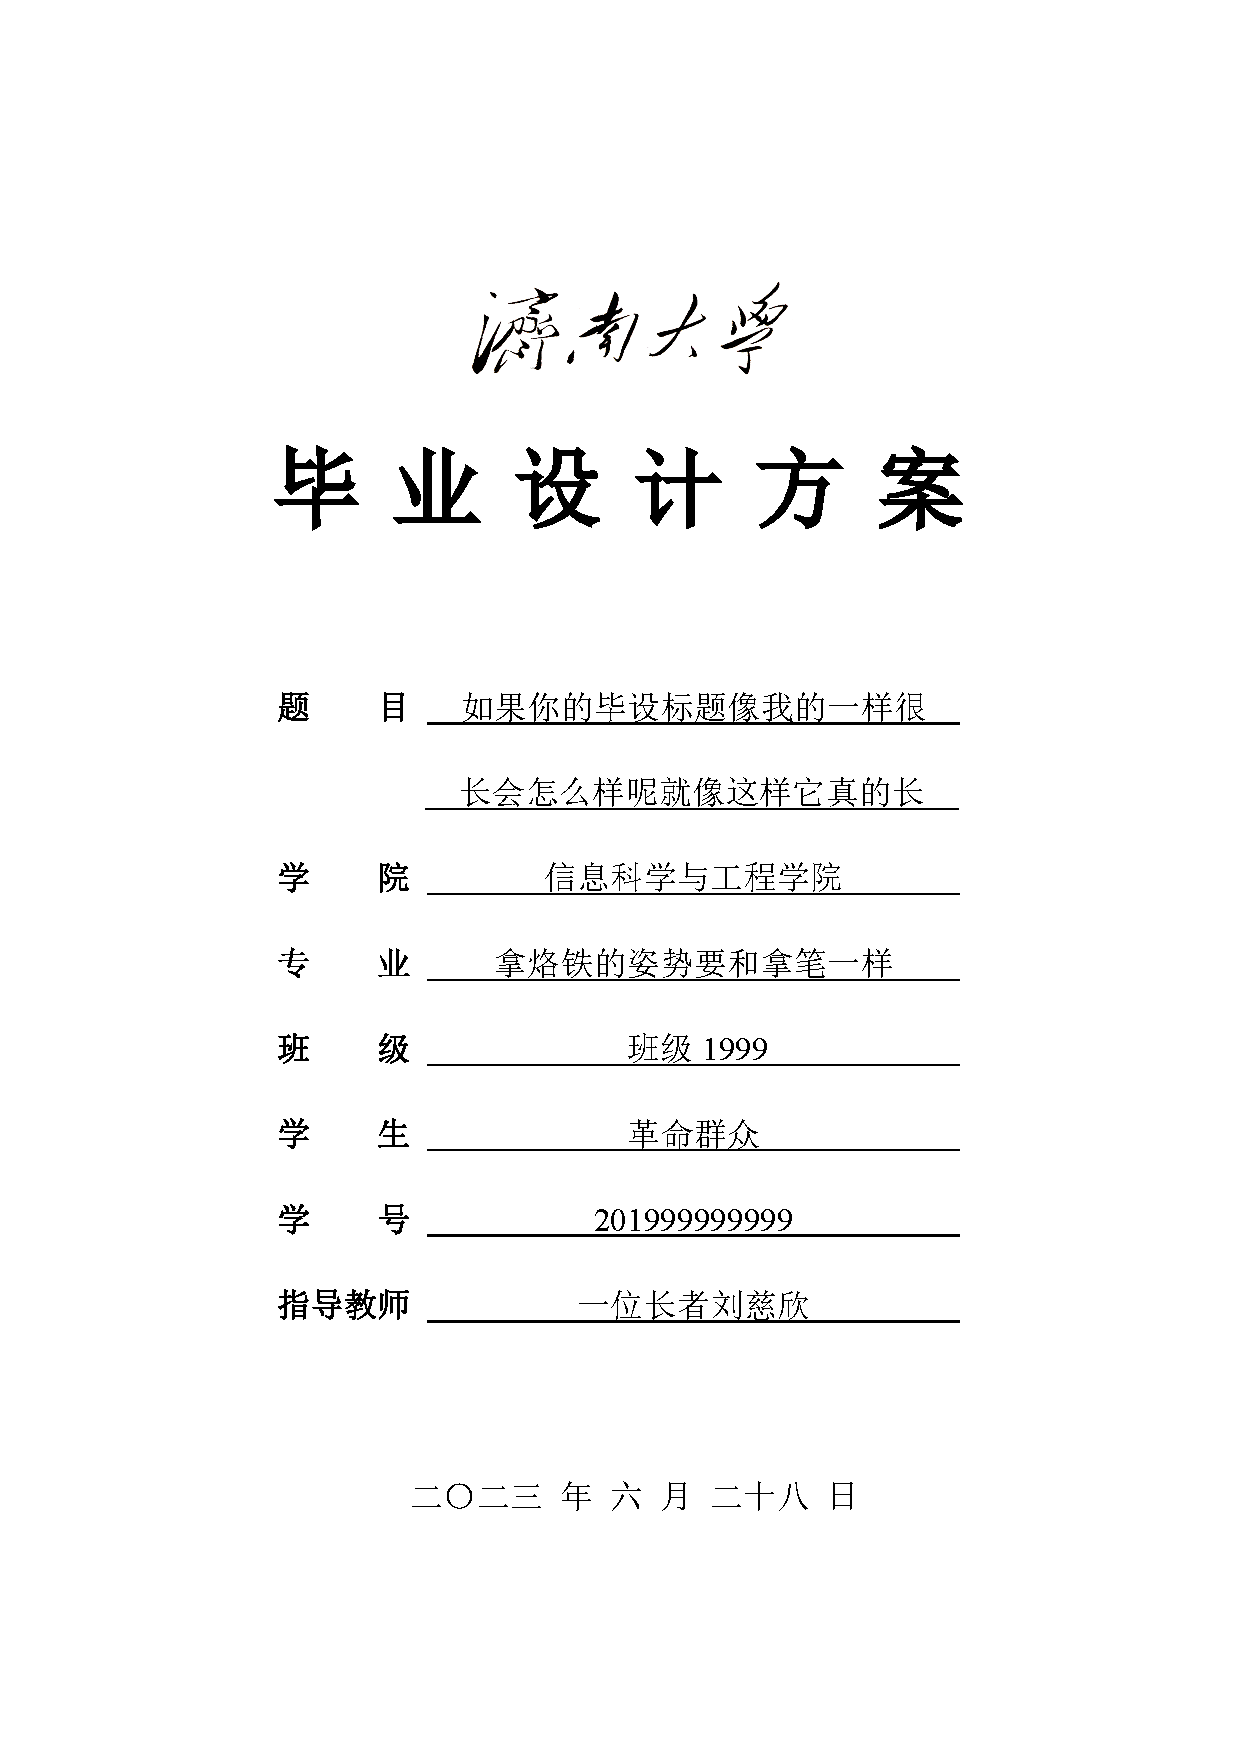
\includepdf[pages=-]{docs/05-report.pdf}
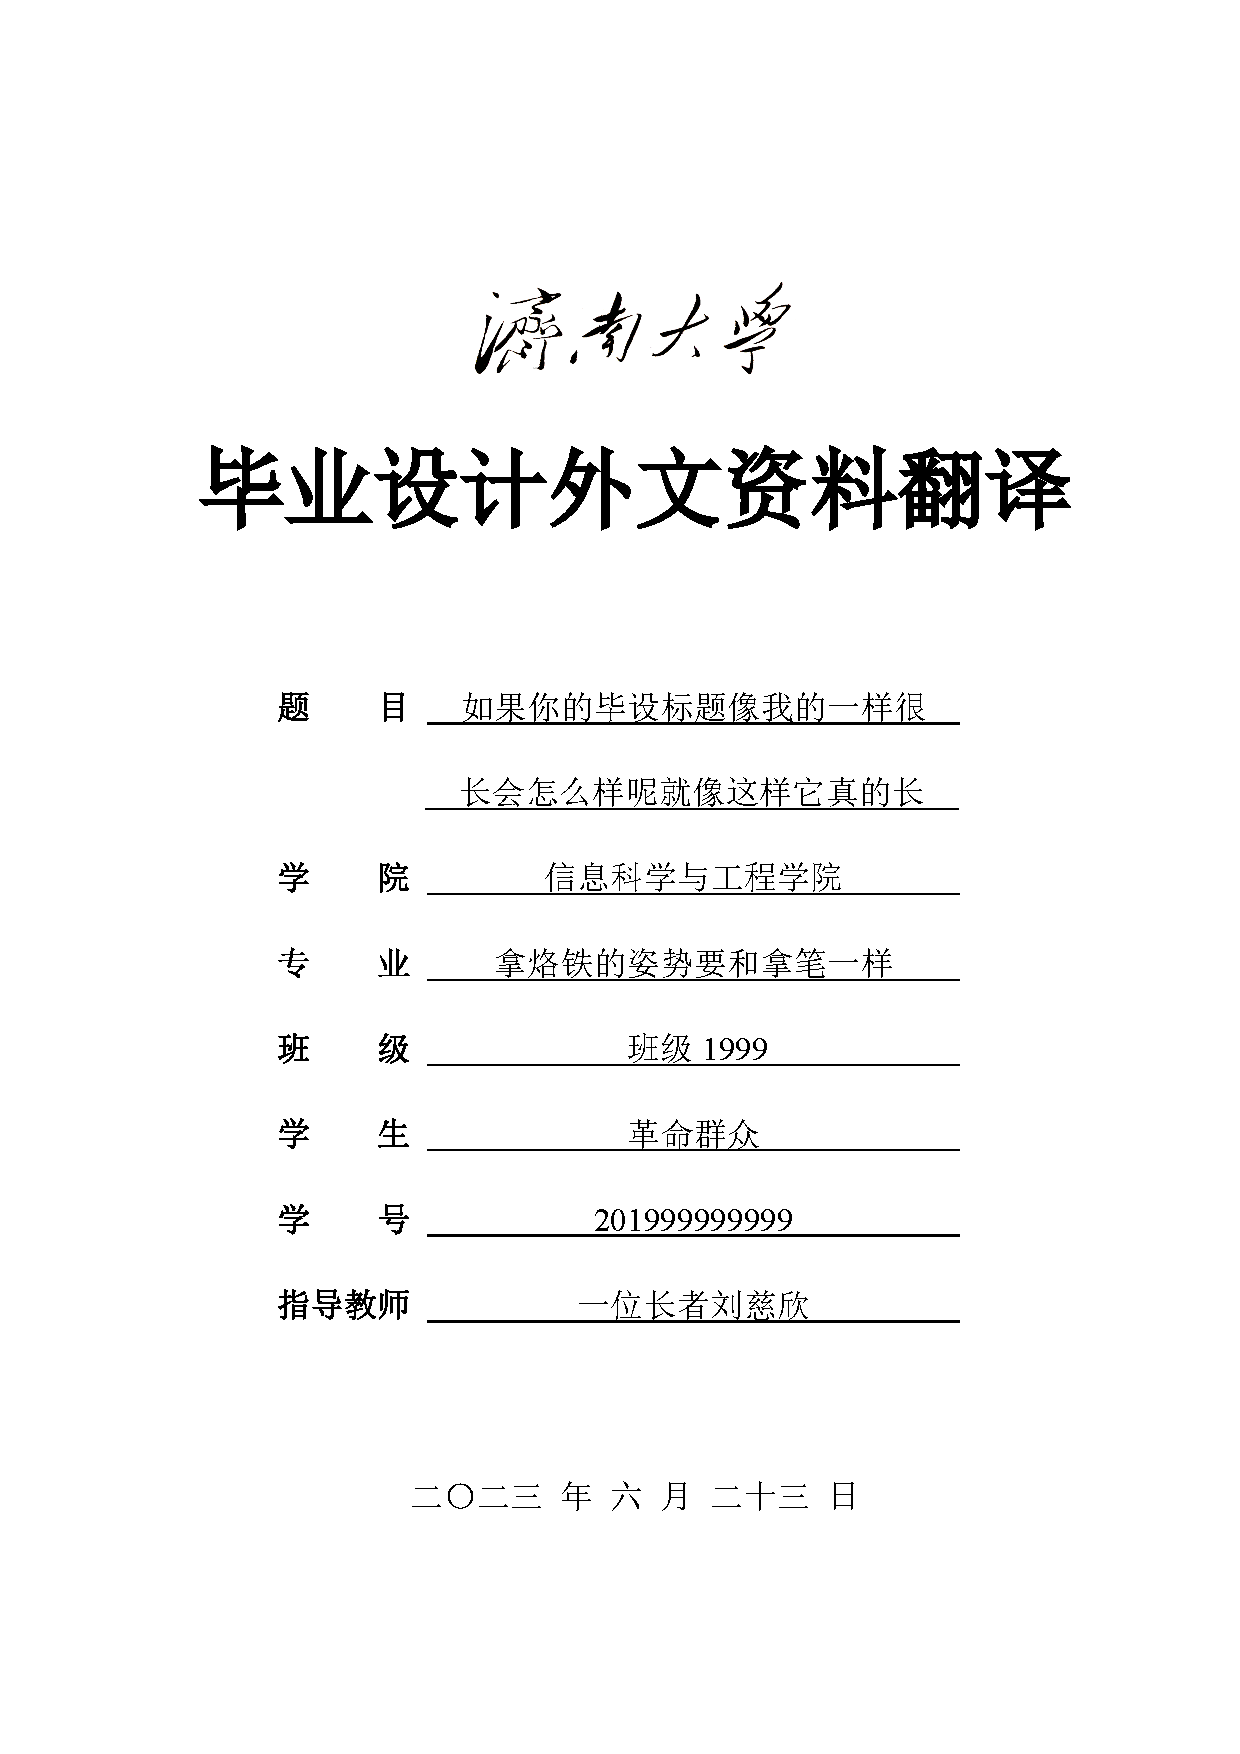
\includepdf[pages=-]{docs/06-cover-translation.pdf}                            % 3-6 表格性质的其他内容
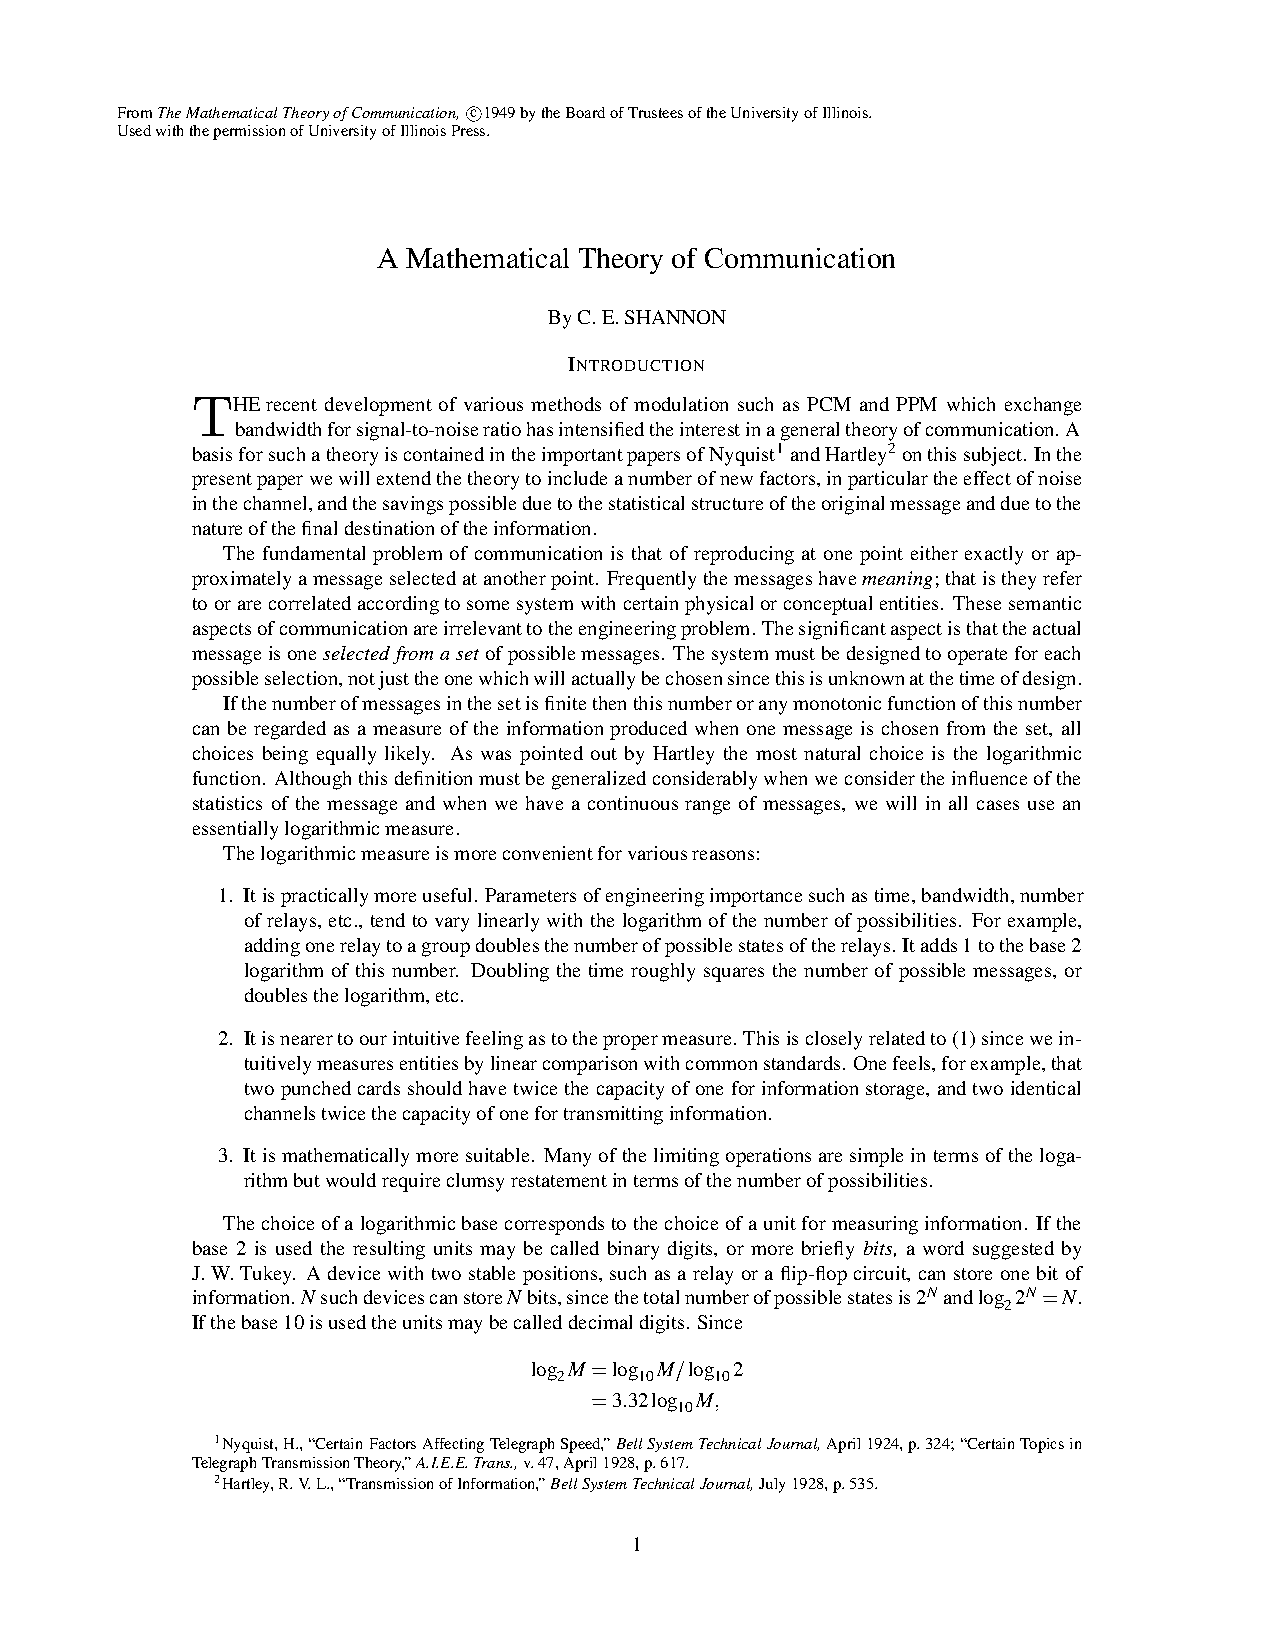
\includepdf[pages=-]{docs/07-text-en.pdf}

当今世界,以信息技术产业为代表的高新技术产业得到了迅猛发展,推动了全球产业结构转型和优化升级,
带来了人类生产生活方式的深刻变化. 进入 21 世纪,信息技术日新月异,
其普及应用对经济、政治、社会、文化、军事发展的影响更加深刻,
信息技术产业已经成为衡量一个国家或地区综合国力、国际竞争力和现代化程度的重要标志。
如何全面把握当代信息技术发展趋势,明确我国未来信息技术产业的发展思路和政策取向,
这是需要我们认真研究和思考的重大问题。

能源是人类生存和发展的重要物质基础,也是当今国际政治、经济、军事、外交关注的焦点。
中国经济社会持续高速发展,离不开有力的能源保障。
在经济全球化深入发展和中国现代化加快推进的大背景下,如何认识能源发展趋势,
选择什么样的能源发展战略,采取什么样的政策措施,是一个非常重要的问题,需要认真加以思考。
                       % 7-8 外文翻译

%%%%%%%%%%%%%%%%%%%%%%%%%%%%%%%% 模板正文 %%%%%%%%%%%%%%%%%%%%%%%%%%%%%%%%%%%

\end{document}
